\documentclass[11pt]{scrartcl}

\title{Anforderungsspezifikation}
\author{Silvan Adrian \\ Fabian Binna}
\date{\today{}}

\usepackage[ngerman]{babel}
\usepackage[automark]{scrpage2}
\usepackage[colorlinks = true,
linkcolor = black]{hyperref}
\usepackage{color}
\usepackage[normalem]{ulem}
\usepackage{scrpage2}
\usepackage{graphicx}
\usepackage{tabularx}
\usepackage{longtable, tabu}
\graphicspath{ {../22_Grafiken/01_Logo/}{images/}{../../22_Grafiken/01_Logo/} }
\pagestyle{scrheadings}

\clearscrheadfoot
\ihead{
\includegraphics[scale=0.3]{SDDC}}
\ohead{Projekt: SDDC}
\ifoot{Anforderungsspezifikation}
\cfoot{Version: 1.06}
\ofoot{Datum: \today{}}
\setheadsepline{0.5pt}
\setfootsepline{0.5pt}

\usepackage{ucs}
\usepackage[utf8]{inputenc}
\usepackage[T1]{fontenc}


\begin{document}
\def\arraystretch{1.5}
\begin{titlepage}
\begin{center}
\vspace{10em}

\includegraphics[scale=2]{SDDC}
\vspace{10em}
\end{center}
\begin{center}
\huge {Anforderungsspezifikation}
\end{center}
\begin{center}
\vspace{10em}
\LARGE {Silvan Adrian} \\
\LARGE {Fabian Binna}
\end{center}

\end{titlepage}

\newpage
\section{Änderungshistorie}
\begin{tabularx}{\linewidth}{l l X l}
\textbf{Datum} & \textbf{Version} & \textbf{Änderung}  & \textbf{Autor} \\
\hline
\textbf{02.10.15} & 1.00 & Erstellung des Dokuments & Gruppe \\
\textbf{02.10.15} & 1.01 & Nicht funktionale Anforderungen & Silvan Adrian\\
\textbf{02.10.15} & 1.02 & Use Cases Aktoren + User Stories Aktoren & Silvan 
Adrian\\
\textbf{03.10.15} & 1.03 & Anforderungen API & Fabian Binna\\
\textbf{03.10.15} & 1.04 & Anforderungen Dashboards + Mockups eingefügt & Silvan 
Adrian\\
\textbf{03.10.15} & 1.05 & Use Cases fully dressed & Silvan Adrian\\
\textbf{04.10.15} & 1.06 & User Stories + NFA's verbessert & Silvan Adrian\\
\end{tabularx}

\newpage
\tableofcontents
\newpage

\section{Einführung}
\subsection{Zweck}
Dieses Dokument beinhaltet die Anforderung zur Analyse.
\subsection{Gültigkeitsbereich}
Dieses Dokument ist während des ganzen Projekts gültig.


\subsection{Referenzen}
-

\section{Anforderungen}
\subsection{API}
Die API definiert einen Workflow der einen Service auf einer Cloud erstellt. Es ist offen, ob 
dieser Service über mehrere Cloud Anbieter hinaus geht. Der Service wird durch 
ein Konfigurationsfile (z.B. json) definiert. Zusätzlich können Scriptfiles referenziert werden, 
die die Software auf den Instanzen installieren. Ein Service kann auch wieder gelöscht werden.
 Es ist nicht die Aufgabe der API existierende Services zu identifizieren. 
 Die API muss Modular sein, das heisst es sollte möglich sein andere oder eigene 
 Programme für die Cloud Kommunikation zu verwenden. Innerhalb der API 
 werden Compute, Storage, Network usw. als ServiceModule bezeichnet. 
 Diese Abstraktion ermöglicht das wiederverwenden und erweitern der API.
\newpage
\subsection{Customer-Dashboard}
\subsubsection{Homescreen}
Im Homescreen (sobald der Customer auf das Dashboard zugreift) werden alle zu 
Verfügung stehenden Services angezeigt.
Hier werden die Services Offerings genannt um eine Unterscheidung zwischen 
Abonnierten Services (Services) und zur Verfügung stehenden Services (Offerings) 
machen zu können.

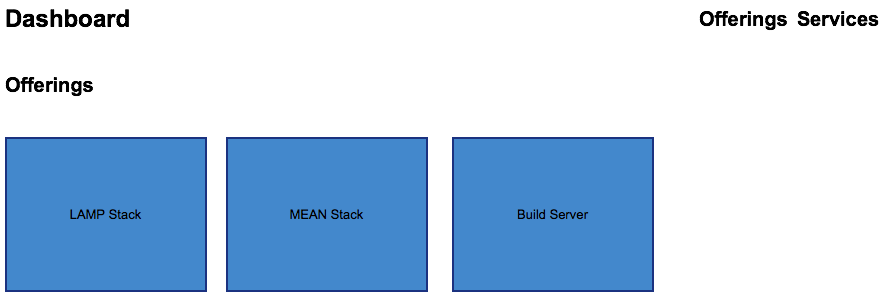
\includegraphics[width=\textwidth]{homescreen_customer}

\subsubsection{Services Übersicht}
In der Services Übersicht werden dem Customer alle abonnierten Services 
angezeigt und können hier auch gekündigt werden.

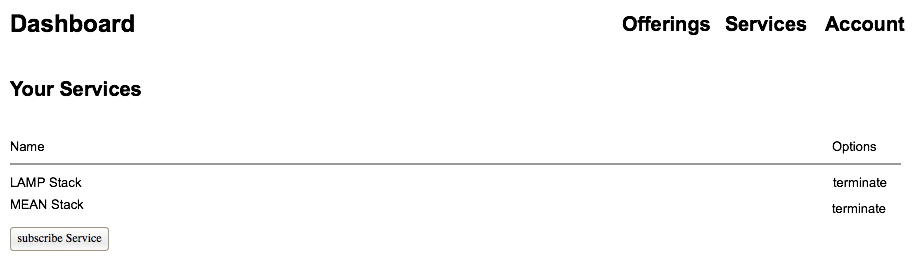
\includegraphics[width=\textwidth]{services_overview}


\subsubsection{Service abonnieren}
Sobald ein Service auf dem Homescreen ausgewählt wird muss noch der zuständige 
Provider gewählt werden (häng auch wieder davon ab von welchem Provider bisher Login Daten hinterlegt 
wurden).
Da momentan noch kein Hybrid Betrieb vorgesehen ist muss ein Account gewählt 
werden unter welchem der Service verrechnet wird.
\begin{figure}[h]
  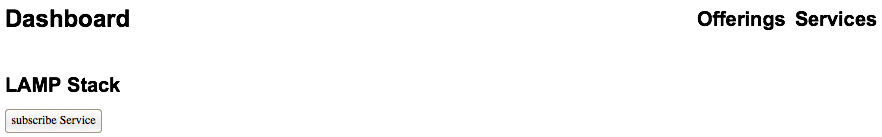
\includegraphics[width=\textwidth]{service_settings}
\end{figure}

\newpage
\subsubsection{Cloud Credentials}
Da für jeden Provider wieder Login Daten benötigt werden müssen diese an einer 
zentralen Stelle gespeichert werden (anhand von denen kann sich auch das Service Angebot 
ändern).
\begin{figure}[h]
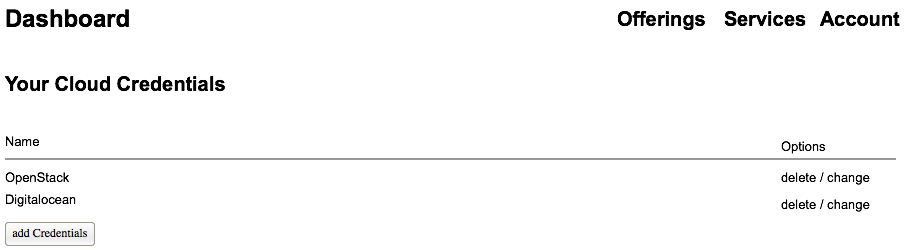
\includegraphics[width=\textwidth]{service_accounts}
\end{figure}
\subsection{Admin-Dashboard}
Zusätzlich zum Customer-Dashboard soll ein Admin-Dashboard zur Verfügung stellen 
in welchem der Admin Services und Servicemodule erstellen kann.

\subsubsection{Service}
Ein Service hat einen bestimmten Namen und jedem Service sind eine gewisse 
Anzahl Servicemodule zugeteilt. um den Service abbilden zu können.
Hier kann der Admin den Service ändern und je nach Anforderung den Service 
anpassen.

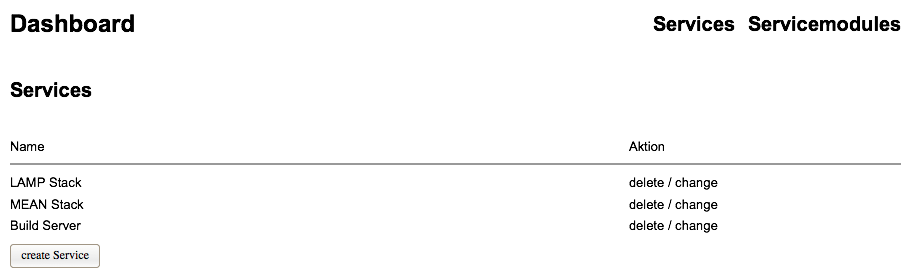
\includegraphics[width=\textwidth]{homescreen_admin}

\subsubsection{Servicemodul}
Jedes Servicemodul besitzt einen Namen und wird einem Provider zugeschrieben, 
dabei kann jedes Servicemodule den Typ Compute,Network oder Storage haben.

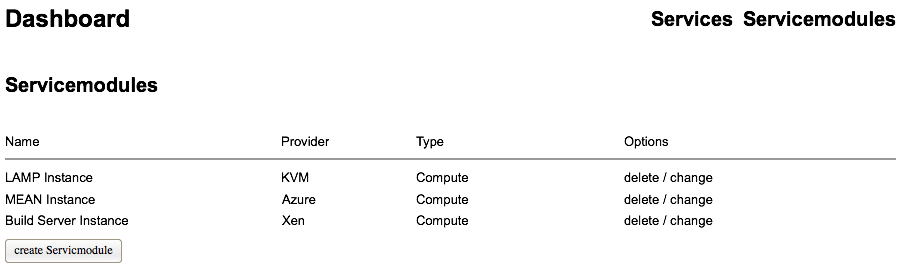
\includegraphics[width=\textwidth]{servicemodules_admin}

\section{Use Cases}
\subsection{Use Case Diagramm}
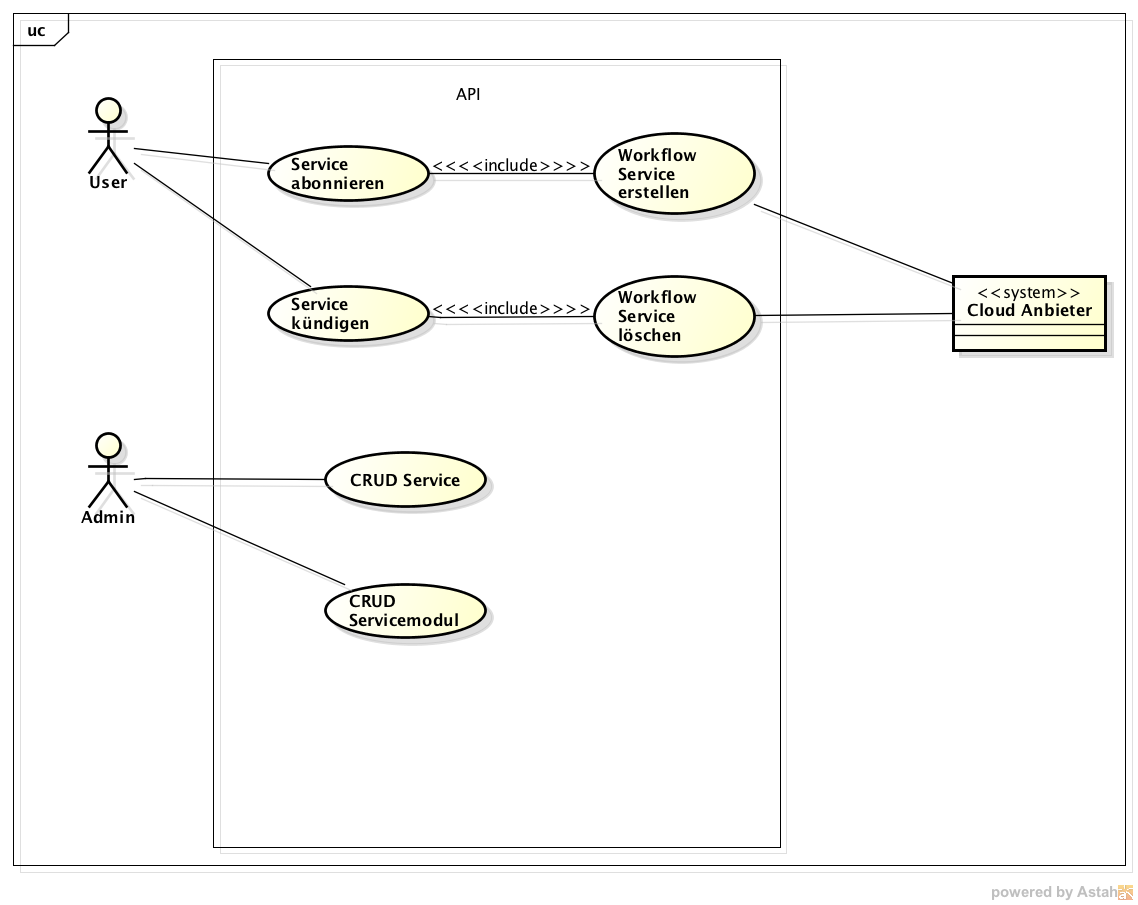
\includegraphics[width=\textwidth]{UseCase-Diagramm}
\subsection{Aktoren \& Stakeholders}
\subsubsection{Customer}
Als Customer möchte ich meine abonnierten Services verwalten.
\\
\begin{tabularx}{\linewidth}{l l X }
  \textbf{Aktor} & \textbf{Typ} & \textbf{Ziele}\\
  \hline
  Customer & Primary & 
  \begin{minipage}{5in}
  \vskip 4pt
  \begin{itemize}
    \item Service abonnieren
    \item Service kündigen
    \item Cloud Login Daten hinzufügen
    \item Cloud Login Daten anpassen
    \item Cloud Login Daten löschen
  \end{itemize}
  \vskip 4pt
 \end{minipage}\\
 \hline
\end{tabularx}


\subsubsection{Admin}
Als Admin möchte ich Services und Servicemodule verwalten können.
\\
\begin{tabularx}{\linewidth}{l l X }
  \textbf{Aktor} & \textbf{Typ} & \textbf{Ziele}\\
  \hline
  Admin & Primary & 
  \begin{minipage}{5in}
  \vskip 4pt
  \begin{itemize}
    \item Service erstellen
    \item Service anpassen
    \item Service löschen
    \item Servicemodul erstellen
    \item Servicemodul anpassen
    \item Servicemodul löschen
  \end{itemize}
  \vskip 4pt
 \end{minipage}\\
 \hline
\end{tabularx}

\newpage
\subsection{Beschreibungen fully dressed}
%Serve abonnieren begin
\subsubsection{UC01: Service abonnieren}
\belowtabulinesep = 1mm
\begin{longtabu} to \textwidth {X[1,l] X[2,l]}
	\bfseries Primäraktor & Customer  \\\hline 
	\bfseries Steakholders und Interessen & Customer: Möchte einen Service abonnieren  \\\hline 
	\bfseries Vorbedingungen & Das Customer-Dashboard wurde geöffnet, ist bei der API authentifiziert und 
	hat einen Cloud Account hinzugefügt. \\\hline 
	\bfseries Nachbedingungen & Die Service Infos wurden gespeichert und der Workflow wurde angestossen  
	\\\hline 
	\bfseries Standartablauf & 
		\begin{enumerate}
			\item Der Customer gibt die Webadresse für das Dashboard ein
			\item Wiederholen bis kein Service mehr abonniert werden soll
			\begin{enumerate}
			    \item Der Customer wechselt in die \textbf{Offerings Übersicht}
			    \item Der Customer wählt einen der vorhanden \textbf{Services} aus
			    \item Der Customer wählt einen vorhanden \textbf{Account} auf welchem er den \textbf{Service}
			abonnieren will
			    \item Der Customer drückt den Button \textbf{subscribe Service}
			    \item Der Customer wird in die \textbf{Services Übersicht} weitergeleitet
			\end{enumerate}
		\item Der Customer schliesst das Customer-Dashboard
		\end{enumerate}
      \\\hline
      	\bfseries Alternativer Ablauf & 
		\begin{enumerate}
		  
		\item
		  \begin{enumerate}
		    \item Der Customer entscheidet sich um und schliesst das 
		    Fenster/Tab
		    
		  \end{enumerate}
		  
		  \item 
                 \begin{enumerate}
		    \item Der Customer entscheidet sich um
		    \begin{enumerate}
		      \item Schliesst das Fenster/Tab
		    \end{enumerate}
		    \item  Der Customer entscheidet sich um
		     \begin{enumerate}
		      \item Schliesst das Fenster/Tab
		      \item geht zurück in die \textbf{Offerings Übersicht}
		    \end{enumerate}
		    
		       \item  Der Customer entscheidet sich um
		     \begin{enumerate}
		      \item Schliesst das Fenster/Tab
		      \item geht zurück in die \textbf{Offerings Übersicht}
		      \item wählt einen anderen Account
		    \end{enumerate}
		    
		    
		     \item  Der Customer entscheidet sich um
		     \begin{enumerate}
		      \item Schliesst das Fenster/Tab
		      \item geht zurück in die \textbf{Offerings Übersicht}
		      \item wählt einen anderen Account
		    \end{enumerate}
		    
		  \end{enumerate}
			
		\end{enumerate}
	 \\\hline
	\bfseries Spezielle Anforderungen & siehe nichtfunktionale Anforderungen  \\\hline 
	\bfseries Technologie- und Datenvarianten & Keine  \\\hline 
	\bfseries Auftrittshäufigkeit & mehrmals pro Woche  \\\hline 
	\bfseries Offene Fragen & Keine  \\\hline  
\end{longtabu}
%Serve abonnieren end
\newpage
%Service kündigen begin
\subsubsection{UC02: Service kündigen}
\begin{longtabu} to \textwidth {X[1,l] X[2,l]}
	\bfseries Primäraktor & Customer  \\\hline 
	\bfseries Steakholders und Interessen & Customer: Möchte einen Service kündigen  \\\hline 
	\bfseries Vorbedingungen & Das Customer-Dashboard wurde geöffnet, ist bei der API authentifiziert und 
	hat einen Service abonniert  \\\hline 
	\bfseries Nachbedingungen & Die Service Infos wurden gelöscht und der Workflow wurde angestossen   \\\hline 
	\bfseries Standartablauf & 
		\begin{enumerate}
			\item Der Customer gibt die Webadresse für das Dashboard ein
			\item Wiederholen bis kein Service mehr gekündigt werden soll
			\begin{enumerate}
			    \item Der Customer wechselt in die \textbf{Services Übersicht}
			    \item Der Customer wählt einen der vorhanden \textbf{Services} aus
			    \item Der Customer drückt auf den link \textbf{terminate}
			    \item Der Customer wird in die \textbf{Services Übersicht} weitergeleitet
			\end{enumerate}
		\item Der Customer schliesst das Customer-Dashboard
		\end{enumerate}
      \\\hline
      	\bfseries Alternativer Ablauf & 
		\begin{enumerate}
		  
		\item
		  \begin{enumerate}
		    \item Der Customer entscheidet sich um und schliesst das 
		    Fenster/Tab
		  \end{enumerate}
		  \item 
                 \begin{enumerate}
		    \item Der Customer entscheidet sich um
		    \begin{enumerate}
		      \item Schliesst das Fenster/Tab
		    \end{enumerate}
		    \item  Der Customer entscheidet sich um
		     \begin{enumerate}
		      \item Schliesst das Fenster/Tab
		      \item wählt einen anderen Service
		    \end{enumerate}
		    
		       \item  Der Customer entscheidet sich um
		     \begin{enumerate}
		      \item Schliesst das Fenster/Tab
		      \item wählt einen anderen Service
		    \end{enumerate}
		    
		  \end{enumerate}
			
		\end{enumerate}
	 \\\hline

      \\\hline
	\bfseries Spezielle Anforderungen & siehe nichtfunktionale Anforderungen  \\\hline 
	\bfseries Technologie- und Datenvarianten & Keine  \\\hline 
	\bfseries Auftrittshäufigkeit & mehrmals pro Woche  \\\hline 
	\bfseries Offene Fragen & Keine  \\\hline  
\end{longtabu}
%Service kündigen end
\newpage
%Cloud Login Daten verwalten begin
\subsubsection{UC03: Cloud Login Daten verwalten}
\begin{longtabu} to \textwidth {X[1,l] X[2,l]}
	\bfseries Primäraktor & Customer  \\\hline 
	\bfseries Steakholders und Interessen & Customer: Möchte ich Cloud Login Daten verwalten  \\\hline 
	\bfseries Vorbedingungen & Das Customer-Dashboard wurde geöffnet  \\\hline 
	\bfseries Nachbedingungen & Die Account Infos wurden gespeichert  \\\hline 
	\bfseries Standartablauf & 
		\begin{enumerate}
			\item Der Customer gibt die Webadresse für das Dashboard ein
			\item Der Customer wechselt in die \textbf{Account/Cloud Credentials Übersicht}
			\item Solange wiederholen bis kein Account mehr hinzugefügt werden muss
			  \begin{enumerate}
			    \item Customer drückt Button \textbf{Add Credentials}
			    \item Customer füllt gefragt Felder aus
			    \item Customer bestätigt Eingaben mit Klick auf \textbf{Save}
			  \end{enumerate}
			\item Der Customer schliesst das Customer-Dashboard
		\end{enumerate}
      \\\hline
      \bfseries Alternativer Ablauf & 
      \begin{enumerate}
          \setcounter{enumi}{2}
            \item 
            \begin{enumerate}
              \item Wiederholen bis kein Account mehr geändert werden muss
                \begin{enumerate}
                  \item Account auswählen und auf \textbf{change} Link klicken
                  \item Felder anpassen
                  \item Änderungen bestätigen mit Klick auf Button \textbf{Save}
                \end{enumerate}
                \item Wiederholen bis kein Account mehr gelöscht werden muss
                \begin{enumerate}
                  \item Account auswählen und auf \textbf{delete} Link klicken
                \end{enumerate}
            \end{enumerate}
            
      \end{enumerate}
      
      \\\hline
	\bfseries Spezielle Anforderungen & siehe nichtfunktionale Anforderungen  \\\hline 
	\bfseries Technologie- und Datenvarianten & Keine  \\\hline 
	\bfseries Auftrittshäufigkeit & mehrmals pro Woche  \\\hline 
	\bfseries Offene Fragen & Keine  \\\hline  
\end{longtabu}
%Cloud Login Daten verwalten end
%Services verwalten begin
\subsubsection{UC04: Services verwalten}

\begin{longtabu} to \textwidth {X[1,l] X[2,l]}
	\bfseries Primäraktor & Customer  \\\hline 
	\bfseries Steakholders und Interessen & Admin: Möchte einen Service verwalten  \\\hline 
	\bfseries Vorbedingungen & Das Admin-Dashboard wurde geöffnet und Admin eingeloggt, 
	falls Service gelöscht werden soll darf kein Customer mehr den Service abonniert haben\\\hline 
	\bfseries Nachbedingungen & Das Admin-Dashboard wurde geschlossen und Änderungen 
	wurden gespeichert  \\\hline 
	\bfseries Standartablauf & 
		\begin{enumerate}
			\item Der Admin gibt die Webadresse für das Admin-Dashboard ein
			\item Wiederholen bis kein neuer Service hinzugefügt werden muss
			\begin{enumerate}
			  \item Der Admin wechselt in die \textbf{Services Übersicht}
			  \item Der Admin drückt auf den button \textbf{create Service}
			  \item Der Admin füllt die benötigten Daten ein \textbf{(Name, welche Servicemodule)}
			  \item der Admin bestätigt mit Klick auf Button \textbf{Save}
			\end{enumerate}
		\end{enumerate}
      \\\hline
      \bfseries Alternativer Ablauf & 
      \begin{enumerate}
        \setcounter{enumi}{1}
        \item 
        \begin{enumerate}
          \item Wiederholen bis kein Service mehr geändert werden muss
            \begin{enumerate}
              \item Service auswählen und auf Link \textbf{change} klicken
              \item Daten ändern
              \item Durch Klick auf Button \textbf{Save} bestätigen
            \end{enumerate}
            \item Wiederholen bis kein Service mehr gelöscht werden muss
            \begin{enumerate}
              \item Service auswählen und Link \textbf{löschen} auswählen
            \end{enumerate}
        \end{enumerate}
      \end{enumerate}
      \\\hline
	\bfseries Spezielle Anforderungen & siehe nichtfunktionale Anforderungen  \\\hline 
	\bfseries Technologie- und Datenvarianten & Keine  \\\hline 
	\bfseries Auftrittshäufigkeit & mehrmals pro Woche  \\\hline 
	\bfseries Offene Fragen & Keine  \\\hline  
\end{longtabu}
%Services verwalten end
\newpage
%Servicemodule verwalten begin
\subsubsection{UC05: Servicemodule verwalten}
\begin{longtabu} to \textwidth {X[1,l] X[2,l]}
	\bfseries Primäraktor & Customer  \\\hline 
	\bfseries Steakholders und Interessen & Admin: Möchte ein Servicemodul verwalten  \\\hline 
	\bfseries Vorbedingungen & Das Admin-Dashboard wurde geöffnet und Admin eingeloggt, 
	falls Servicemodul gelöscht werden soll darf kein Service mehr das Servicemodul verwenden. \\\hline 
	\bfseries Nachbedingungen & Das Admin-Dashboard wurde geschlossen und 
	Änderungen wurden gespeichert \\\hline 
	\bfseries Standartablauf & 
	\begin{enumerate}
			\item Der Admin gibt die Webadresse für das Admin-Dashboard ein
			\item Wiederholen bis kein neues Servicemodul hinzugefügt werden muss
			\begin{enumerate}
			  \item Der Admin wechselt in die \textbf{Servicemodules Übersicht}
			  \item Der Admin drückt auf den button \textbf{create Servicemodule}
			  \item Der Admin füllt die benötigten Daten ein \textbf{(Name, Provider,Typ)}
			  \item der Admin bestätigt mit Klick auf Button \textbf{Save}
			\end{enumerate}
		\end{enumerate}
      \\\hline
      \bfseries Alternativer Ablauf & 
      \begin{enumerate}
        \setcounter{enumi}{1}
        \item 
        \begin{enumerate}
          \item Wiederholen bis kein Servicemodul mehr geändert werden muss
            \begin{enumerate}
              \item Servicemodul auswählen und auf Link \textbf{change} klicken
              \item Daten ändern
              \item Durch Klick auf Button \textbf{Save} bestätigen
            \end{enumerate}
            \item Wiederholen bis kein Servicemodul mehr gelöscht werden muss
            \begin{enumerate}
              \item Service auswählen und Link \textbf{löschen} auswählen
            \end{enumerate}
        \end{enumerate}
      \end{enumerate}
      \\\hline

	\bfseries Spezielle Anforderungen & siehe nichtfunktionale Anforderungen  \\\hline 
	\bfseries Technologie- und Datenvarianten & Keine  \\\hline 
	\bfseries Auftrittshäufigkeit & mehrmals pro Woche  \\\hline 
	\bfseries Offene Fragen & Keine  \\\hline  
\end{longtabu}
%Servicemodule verwalten end


\newpage
\section{Epics}
\subsection{Customer}
\begin{itemize}
  \item Service abonnieren
  \item Service kündigen
  \item Cloud Login Daten verwalten
\end{itemize}
\subsection{Admin}
\begin{itemize}
  \item Service verwalten
  \item Servicemodul verwalten
\end{itemize}
\section{User Stories}
\subsection{Rollen}
\subsubsection{Customer}
Als Customer benutze ich das Dashboard, um für mich einen Service zu abonnieren oder zu 
kündigen, ebenfalls verwalte ich meine Cloud Login Daten
\subsubsection{Admin}
Als Admin erstelle ich neue Services und Servicemodule und erweitere diese um 
neue Funktionen/Verbesserungen.
\subsection{Customer}
\subsubsection{Customer greift auf Customer-Dashboard zu}
\begin{tabularx}{\linewidth}{l X}
  \textbf{Priorität} & Niedrig\\
  \hline
  \textbf{Story Points} & 1\\
  \hline
  \textbf{Story}& Als Customer möchte ich auf das Customer-Dashboard zugreifen können\\
  \hline
    \textbf{Akzeptanzkriterien} & \\
    \hline
  \textbf{A1} & Der Customer kann den Url des Customer-Dashboard aufrufen und 
  kriegt das Dashboard angezeigt\\
  \hline
   \end{tabularx}
   
 \subsubsection{Customer geht in die Offerings Übersicht}
\begin{tabularx}{\linewidth}{l X}
  \textbf{Priorität} & Niedrig\\
  \hline
  \textbf{Story Points} & 2\\
  \hline
  \textbf{Story}& Als Customer möchte ich die Offerings in einer Übersicht ansehen können\\
  \hline
    \textbf{Akzeptanzkriterien} & \\
    \hline
  \textbf{A1} & Der Customer kann im Dashboard in die Offerings Übersicht wechseln.\\
  \hline
   \end{tabularx}
   
 \subsubsection{Customer geht in die Service Übersicht}
\begin{tabularx}{\linewidth}{l X}
  \textbf{Priorität} & Niedrig\\
  \hline
  \textbf{Story Points} & 2\\
  \hline
  \textbf{Story}& Als Customer möchte ich meine abonnierten Services in einer Übersicht angezeigt bekommen\\
  \hline
    \textbf{Akzeptanzkriterien} & \\
    \hline
  \textbf{A1} & Der Customer kann seine abonnierten Services in einer Übersicht anzeigen\\
  \hline
   \end{tabularx}
   
 \subsubsection{Customer fügt Cloud Login Daten hinzu}
\begin{tabularx}{\linewidth}{l X}
  \textbf{Priorität} & Mittel\\
  \hline
  \textbf{Story Points} & 3\\
  \hline
  \textbf{Story}& Als Customer möchte ich meine Cloud Login Daten meinem Account hinterlegen\\
  \hline
    \textbf{Akzeptanzkriterien} & \\
    \hline
  \textbf{A1} & Der Customer kann seine Login Daten hinzufügen\\
  \hline
  \textbf{A2} & In der Offerings Übersicht werden die neuen möglichen Services 
  angezeigt\\
  \hline
    \textbf{A3} & Die neuen Login Daten werden gespeichert\\
  \hline
   \end{tabularx}
 \subsubsection{Customer ändert Cloud Login Daten}
\begin{tabularx}{\linewidth}{l X}
  \textbf{Priorität} & Mittel\\
  \hline
  \textbf{Story Points} & 3\\
  \hline
  \textbf{Story}& Als Customer möchte ich meine hinterlegten Cloud Login Daten ändern können\\
  \hline
    \textbf{Akzeptanzkriterien} & \\
    \hline
  \textbf{A1} & Der Customer kann seine Login Daten ändern\\
  \hline
    \textbf{A2} & Die Änderungen werden gespeichert\\
  \hline
   \end{tabularx}
 \subsubsection{Customer löscht Cloud Login Daten}
\begin{tabularx}{\linewidth}{l X}
  \textbf{Priorität} & Mittel\\
  \hline
  \textbf{Story Points} & 4\\
  \hline
  \textbf{Story}& Als Customer möchte ich meine Cloud Login Daten aus meinem Account entfernen können\\
  \hline
    \textbf{Akzeptanzkriterien} & \\
    \hline
  \textbf{A1} & Der Customer kann seine Login Daten löschen\\
  \hline
  \textbf{A2} & Account kann nicht gelöscht werden, falls noch abonnierte Services auf dem Account bestehen\\
  \hline
    \textbf{A3} & Die Login Daten werden entfernt\\
  \hline
   \end{tabularx}
 \subsubsection{Customer abonniert Service}
\begin{tabularx}{\linewidth}{l X}
  \textbf{Priorität} & Hoch\\
  \hline
  \textbf{Story Points} & 6\\
  \hline
  \textbf{Story}& Als Customer möchte ich einen Service abonnieren können\\
  \hline
    \textbf{Akzeptanzkriterien} & \\
    \hline
  \textbf{A1} & Der Customer kann einen Service abonnieren\\
  \hline
  \textbf{A2} & Service wird in die Service Übersicht aufgenommen\\
  \hline
    \textbf{A3} & Storage,Compute und Network wurden, wie im Service beschrieben erstellt\\
  \hline
      \textbf{A4} & Neuere Version des Services kann nicht abonniert werden wenn alte Version noch abonniert ist\\
  \hline
   \end{tabularx}
 \subsubsection{Customer kündigt Service}
 \begin{tabularx}{\linewidth}{l X}
     \textbf{Priorität} & Hoch\\
  \hline
  \textbf{Story Points} & 6\\
  \hline
  \textbf{Story}& Als Customer möchte ich einen Service kündigen können\\
  \hline
    \textbf{Akzeptanzkriterien} & \\
    \hline
  \textbf{A1} & Der Customer kann einen Service kündigen\\
  \hline
  \textbf{A2} & Service wird aus der Service Übersicht entfernt\\
  \hline
    \textbf{A3} & Storage,Compute und Network werden, wie im Service beschrieben gelöscht\\
  \hline
      \textbf{A4} & Service wird wieder in der Offerings Übersicht angezeigt in seiner neusten Version\\
  \hline
   \end{tabularx}
  
 \subsection{Admin}
 \subsubsection{Admin greift auf Dashboard zu}
\begin{tabularx}{\linewidth}{l X}
  \textbf{Priorität} & Hoch\\
  \hline
  \textbf{Story Points} & 1\\
  \hline
  \textbf{Story}& Als Admin möchte ich auf das Admin-Dashboard zugreifen können\\
  \hline
    \textbf{Akzeptanzkriterien} & \\
    \hline
  \textbf{A1} & Der Admin kann den Url des Customer-Dashboard aufrufen und 
  kriegt ein Login angezeigt.\\
  \hline
  \textbf{A2} & Der Admin kann sich einloggen und kriegt die Service Übersicht angezeigt\\
  \hline
 \end{tabularx}
 
 
  \subsubsection{Admin erstellt Servicemodul}
\begin{tabularx}{\linewidth}{l X}
  \textbf{Priorität} & Hoch\\
  \hline
  \textbf{Story Points} & 4\\
  \hline
  \textbf{Story}& Als Admin möchte ich Servicemodule erstellen können\\
  \hline
    \textbf{Akzeptanzkriterien} & \\
    \hline
  \textbf{A1} & Das Servicemodule kann nur erstellt werden, falls Admin eingeloggt ist.\\
  \hline
  \textbf{A2} & Das Servicemodul wird erstellt und wird in der Servicemodule Übersicht angezeigt\\
  \hline
 \end{tabularx}
 
   \subsubsection{Admin ändert Servicemodul}
\begin{tabularx}{\linewidth}{l X}
  \textbf{Priorität} & Hoch\\
  \hline
  \textbf{Story Points} & 4\\
  \hline
  \textbf{Story}& Als Admin möchte ich Servicemodule ändern können\\
  \hline
    \textbf{Akzeptanzkriterien} & \\
    \hline
      \textbf{A1} & Das Servicemodule kann nur geändert werden, falls Admin eingeloggt ist.\\
  \hline
  \textbf{A2} & Als Admin krieg ich die Übersicht der verfügbaren Servicemodule\\
  \hline
  \textbf{A3} & Als Admin kann ich Name, Provider anpassen und speichern\\
  \hline
    \textbf{A4} & Versionsnummer des Servicemoduls ändert sich\\
  \hline
    \textbf{A5} & Änderungen werden gespeichert\\
  \hline
 \end{tabularx}
 
 
 \subsubsection{Admin löscht Servicemodul}
 
 \begin{tabularx}{\linewidth}{l X}
  \textbf{Priorität} & Hoch\\
  \hline
  \textbf{Story Points} & 4\\
  \hline
  \textbf{Story}& Als Admin möchte ich Servicemodule löschen können\\
  \hline
    \textbf{Akzeptanzkriterien} & \\
    \hline
      \textbf{A1} & Das Servicemodule kann nur gelöscht werden, falls Admin eingeloggt ist.\\
  \hline
  \textbf{A2} & Als Admin krieg ich die Übersicht der verfügbaren Servicemodule\\
  \hline
  \textbf{A3} & Servicemodule kann gelöscht werden, falls kein Service das Modul mehr nutzt\\
  \hline
    \textbf{A4} & Servicemodule ist gelöscht\\
  \hline
 \end{tabularx}
 
 
 \subsubsection{Admin erstellt Service}
 \begin{tabularx}{\linewidth}{l X}
  \textbf{Priorität} & Hoch\\
  \hline
  \textbf{Story Points} & 6\\
  \hline
  \textbf{Story}& Als Admin möchte ich Services erstellen können\\
  \hline
    \textbf{Akzeptanzkriterien} & \\
    \hline
      \textbf{A1} & Der Service kann nur erstellt werden, falls Admin eingeloggt ist.\\
  \hline
  \textbf{A2} & Als Admin krieg ich die Übersicht der verfügbaren Services\\
  \hline
    \textbf{A3} & Dem Service können Servicemodule hinzugefügt werden\\
  \hline
  \textbf{A4} & Service kann erstellt werden\\
  \hline
    \textbf{A5} & Der Service ist erstellt\\
  \hline
 \end{tabularx}
 
 \subsubsection{Admin ändert Service}
 \begin{tabularx}{\linewidth}{l X}
  \textbf{Priorität} & Hoch\\
  \hline
  \textbf{Story Points} & 6\\
  \hline
  \textbf{Story}& Als Admin möchte ich Services ändern können\\
  \hline
    \textbf{Akzeptanzkriterien} & \\
    \hline
      \textbf{A1} & Der Service kann nur geändert werden, falls Admin eingeloggt ist.\\
  \hline
  \textbf{A2} & Als Admin krieg ich die Übersicht der verfügbaren Services\\
  \hline
    \textbf{A3} & Dem Service können Servicemodule hinzugefügt werden\\
  \hline
  \textbf{A4} & Service kann geändert werden\\
  \hline
    \textbf{A5} & Der Service ist geändert\\
  \hline
  \textbf{A6} & Der Service wird als neue Version gespeichert\\
  \hline
 \end{tabularx}

 \subsubsection{Admin löscht Service}
 
  \begin{tabularx}{\linewidth}{l X}
  \textbf{Priorität} & Hoch\\
  \hline
  \textbf{Story Points} & 6\\
  \hline
  \textbf{Story}& Als Admin möchte ich Services löschen können\\
  \hline
    \textbf{Akzeptanzkriterien} & \\
    \hline
      \textbf{A1} & Der Service kann nur gelöscht werden, falls Admin eingeloggt ist.\\
  \hline
  \textbf{A2} & Als Admin krieg ich die Übersicht der verfügbaren Services\\
  \hline
  \textbf{A4} & Service kann gelöscht werden, falls niemand mehr den Service abonniert hat\\
  \hline
    \textbf{A5} & Der Service ist gelöscht\\
  \hline
 \end{tabularx}
 
 \subsubsection{Admin Login ins Admin Dashboard}
   \begin{tabularx}{\linewidth}{l X}
  \textbf{Priorität} & Hoch\\
  \hline
  \textbf{Story Points} & 2\\
  \hline
  \textbf{Story}& Als Admin möchte ich mich ins Admin-Dashboard einloggen können\\
  \hline
    \textbf{Akzeptanzkriterien} & \\
    \hline
      \textbf{A1} & Der Admin kann sich einloggen\\
  \hline
 \end{tabularx}

 \subsubsection{Admin geht in die Service Übersicht}
 
    \begin{tabularx}{\linewidth}{l X}
  \textbf{Priorität} & Hoch\\
  \hline
  \textbf{Story Points} & 2\\
  \hline
  \textbf{Story}& Als Admin möchte ich einen Überblick über die vorhanden Services\\
  \hline
    \textbf{Akzeptanzkriterien} & \\
    \hline
      \textbf{A1} & Der Admin kann die Service Übersicht öffnen\\
  \hline
    \textbf{A2} & Die Service Übersicht wird nur angezeigt, falls der Admin eingeloggt ist.\\
  \hline
 \end{tabularx}

 \subsubsection{Admin geht in die Servicemodul Übersicht}
 
     \begin{tabularx}{\linewidth}{l X}
  \textbf{Priorität} & Hoch\\
  \hline
  \textbf{Story Points} & 2\\
  \hline
  \textbf{Story}& Als Admin möchte ich einen Überblick über die vorhanden Servicemodule\\
  \hline
    \textbf{Akzeptanzkriterien} & \\
    \hline
      \textbf{A1} & Der Admin kann die Servicemodule Übersicht öffnen\\
  \hline
    \textbf{A2} & Die Servicemodule Übersicht wird nur angezeigt, falls der Admin eingeloggt ist.\\
  \hline
 \end{tabularx}


 \subsubsection{Admin Konfigurationsdatei im Servicemodul hinterlegen}
     \begin{tabularx}{\linewidth}{l X}
  \textbf{Priorität} & Hoch\\
  \hline
  \textbf{Story Points} & 2\\
  \hline
  \textbf{Story}& Als Admin möchte ich dem Servicemodul eine Konfigurationsdatei hinterlegen\\
  \hline
    \textbf{Akzeptanzkriterien} & \\
    \hline
      \textbf{A1} & Der Admin kann dem Servicemodul eine Konfigurationsdatei hinterlegen\\
  \hline
    \textbf{A2} & Die Konfigurationsdatei kann nur hinterlegt werden, falls der Admin eingeloggt ist.\\
  \hline
 \end{tabularx}

\newpage

\section{Nicht-funktionale Anforderungen}
\subsection{Menge}
\begin{itemize}
  \item Die Software unterstützt mehr als 30 Cloud Anbieter (libcloud)
  \item Bei jedem Cloud Anbieter bestehen eine gewisse Anzahl Services (von Anbieter zu Anbieter verschieden)
\end{itemize}

\subsection{Schnittstellen}
\begin{itemize}
  \item Die Software wird über HTTP/HTTPS angesprochen
  \item Zur Interaktion im Admin-Dashboard/Customer-Dashboard werden die herkömmlichen 
  Schnittstellen gebraucht (Maus,Tastatur,Bildschirm)
\end{itemize}
\subsection{Qualitätsmerkmale}
\subsubsection{Funktionalität}
siehe Abschnitt API und Dashboard
\subsubsection{Zuverlässigkeit}
\begin{itemize}
  \item Der Workflow zum erstellen eines Services soll entweder durchgeführt und 
  abgeschlossen werden oder falls Unterbruch/Fehler rückgängig gemacht 
  werden.
  \item Die Software soll verteilt betrieben werden und eine möglichst hohe 
  Verfügbarkeit/Zuverlässigkeit bieten
\end{itemize}
\subsubsection{Benutzerbarkeit}
\begin{itemize}
  \item Konfigurationen können über das vorgesehene Admin-Dashboard benutzt werden
  \item Zum verwenden der Software besteht noch ein einfaches 
  User-Dashboard
\end{itemize}
\subsubsection{Effizienz}
\begin{itemize}
  \item Die Software Soll mehrere Aufträge von Customern gleichzeitig abarbeiten können
\end{itemize}
\subsubsection{Änderbarkeit}
Die Software soll modular aufgebaut werden, damit Erweiterungen in Zukunft 
problemlos möglich sind.
\subsubsection{Übertragbarkeit}
Das Projekt wird in Python geschrieben ist somit also auf Python mindestens in der Version 2.5 angewiesen, 
kann allerdings durch den Einsatz eines Docker Containers einfach Übertragbar 
gemacht werden.
\end{document}